\documentclass[11pt]{article}

% Packages
\usepackage[margin=1.2in]{geometry}
\usepackage{amsmath,amssymb,amsthm,mathtools}
\usepackage{graphicx}
\usepackage{booktabs}
\usepackage{caption}
\usepackage{float}
\usepackage{hyperref}

% Theorem Environments (Unified Counter)
\newtheorem{theorem}{Theorem}[section]
\newtheorem{definition}[theorem]{Definition}
\newtheorem{proposition}[theorem]{Proposition}
\newtheorem{corollary}[theorem]{Corollary}

% Shortcuts
\newcommand{\T}{\mathbb{T}}

% Title
\title{Transient Rational Locking in Modular Logarithmic Orbits}
\author{jhuckstead83\\\small \url{https://github.com/jhuckstead83}\\\small \url{https://orcid.org/0009-0007-0234-2177}}
\date{}

\begin{document}

\maketitle

\begin{abstract}
Apparent geometric skeletons in modular logarithmic orbits are not fundamental structural properties of the constants themselves. They are transient, predictable manifestations of exact rational shadowing. This paper demonstrates that apparent $q$-sector symmetries are governed entirely by strong rational approximants to the rotation number, with visual persistence dictated by a periodic torus-sawtooth dephasing law. The discrete modulus acts strictly as a rendering lens, amplifying or blurring the intrinsic geometry based on arithmetic commensurability, but composing none of it.
\end{abstract}

\vspace{0.4cm}

\section{Definitions}

Let $\alpha,\beta>0$ with $\beta\neq 1$. We define the associated \textbf{rotation number}
\begin{equation}
\rho(\alpha;\beta)
=
\left\{\frac{\log \alpha}{\log \beta}\right\}
\in [0,1),
\end{equation}
where $\{x\}=x-\lfloor x\rfloor$ denotes the fractional part. This quantity determines a rigid rotation on the one-dimensional torus
\[
\T=\mathbb{R}/\mathbb{Z}.
\]

\begin{definition}[Modular logarithmic orbit]
Given $\rho=\rho(\alpha;\beta)$, define the orbit
\[
x_n=\{n\rho\}, \qquad n\ge 1.
\]
We refer to $(x_n)_{n\ge 1}$ as the \emph{modular logarithmic orbit} generated by the pair $(\alpha,\beta)$.
\end{definition}

This orbit is the primary object of study. Geometric patterns observed in modular projections are interpreted as properties of this rotation sequence.

\begin{definition}[Rational carrier]
Let $p/q\in [0,1)$ be a reduced rational number with $q\ge 1$. The associated \textbf{rational carrier} is the periodic sequence
\[
c_n^{(p/q)}=\left\{\frac{np}{q}\right\}, \qquad n\ge 1.
\]
\end{definition}

Since $p/q$ is rational, the carrier has exact period $q$ on $\T$, and its image is the $q$-point lattice
\[
\left\{0,\frac{1}{q},\frac{2}{q},\dots,\frac{q-1}{q}\right\}
\]
up to permutation. When $\rho$ is close to $p/q$, the orbit $x_n$ may temporarily shadow this exact $q$-sector structure.

\begin{definition}[Dephasing error]
Given a rational approximant $p/q$ to $\rho$, define the signed \textbf{dephasing error} relative to the carrier $p/q$ by
\[
\delta=\rho-\frac{p}{q}.
\]
\end{definition}

This decomposition yields
\[
\rho=\frac{p}{q}+\delta,
\]
and therefore
\[
x_n
=
\{n\rho\}
=
\left\{\frac{np}{q}+n\delta\right\}.
\]
The orbit is thus naturally interpreted as an exact rational carrier modulated by a linearly accumulating phase drift.

\begin{definition}[Torus distance]
For $u,v\in \T$, define the circular distance
\[
d_{\T}(u,v)=\min\bigl(|u-v|,\ 1-|u-v|\bigr).
\]
\end{definition}

Using this metric, we define the \textbf{carrier-tracking error}
\begin{equation}
\epsilon_n^{(p/q)}
=
d_{\T}\!\left(x_n,\ c_n^{(p/q)}\right).
\end{equation}
This quantity measures how closely the orbit shadows the moving rational carrier at time $n$.

\begin{definition}[Lock scale]
For a nonzero dephasing error $\delta$, define the nominal \textbf{lock scale}
\[
N_{\mathrm{lock}}=\frac{1}{|\delta|}.
\]
\end{definition}

This scale will not be interpreted as a terminal breakdown time. Rather, it is the natural period associated with the dephasing cycle on the torus.

\begin{definition}[Discretized lane projection]
For a modulus $M\in\mathbb{N}$, define the lane projection of $x_n$ by
\[
\ell_n^{(M)}=\left\lfloor Mx_n\right\rfloor \in \{0,1,\dots,M-1\}.
\]
Similarly, for the carrier $c_n^{(p/q)}$, define
\[
\ell_{n,\mathrm{car}}^{(M)}=
\left\lfloor M\,c_n^{(p/q)}\right\rfloor.
\]
\end{definition}

These discretized projections depend on the chosen modulus $M$. They are therefore regarded as rendering coordinates rather than intrinsic dynamical quantities.

\begin{definition}[Normalized lane error]
The circular lane distance between two residues $a,b\in\{0,\dots,M-1\}$ is
\[
d_M(a,b)=\frac{1}{M}\min(|a-b|,\ M-|a-b|).
\]
The corresponding normalized lane error at time $n$ is
\[
\lambda_n^{(M,p/q)}
=
d_M\!\left(\ell_n^{(M)},\ \ell_{n,\mathrm{car}}^{(M)}\right).
\]
\end{definition}

This quantity measures how the rational shadowing appears after discretization by modulus $M$. The distinction between $\epsilon_n^{(p/q)}$ and $\lambda_n^{(M,p/q)}$ is fundamental:
\begin{itemize}
    \item $\epsilon_n^{(p/q)}$ is intrinsic to the orbit on the torus,
    \item $\lambda_n^{(M,p/q)}$ depends on the observing modulus.
\end{itemize}

\section{The Dephasing Law}

We now derive the basic mechanism underlying transient rational locking.

Let
\[
\rho=\frac{p}{q}+\delta
\]
for some rational approximant $p/q$. Then the orbit satisfies
\[
x_n
=
\{n\rho\}
=
\left\{\frac{np}{q}+n\delta\right\}.
\]
The first term is the exact rational carrier, while the second is a cumulative drift term.

\begin{proposition}[Exact carrier-shadowing formula]
Let $x_n=\{n\rho\}$ and $c_n^{(p/q)}=\{np/q\}$. Then
\begin{equation}
\epsilon_n^{(p/q)}
=
d_{\T}\!\left(x_n,c_n^{(p/q)}\right)
=
\lVert n\delta\rVert_{\T},
\end{equation}
where
\[
\lVert y\rVert_{\T}=\min_{k\in\mathbb{Z}}|y-k|
\]
denotes distance to the nearest integer.
\end{proposition}

\begin{proof}
Using $\rho=p/q+\delta$,
\[
x_n
=
\left\{n\left(\frac{p}{q}+\delta\right)\right\}
=
\left\{\frac{np}{q}+n\delta\right\}.
\]
Subtracting the carrier $c_n^{(p/q)}=\{np/q\}$ on the torus leaves precisely the class of $n\delta$ modulo $1$. Hence
\[
d_{\T}\!\left(x_n,c_n^{(p/q)}\right)=\lVert n\delta\rVert_{\T}.
\]
\end{proof}

This identity is the central mechanical law. Apparent geometric locking is exactly the statement that the orbit remains close to its rational carrier under the torus metric.

The formula
\[
\epsilon_n^{(p/q)}=\lVert n\delta\rVert_{\T}
\]
shows that the orbit does not merely stay near a static $q$-sector lattice. It tracks a moving rational target whose phase error increases linearly in $n$, then wraps around modulo $1$. Thus the relevant dynamics are not binary, such as ``locked'' versus ``broken,'' but cyclic:
\begin{itemize}
    \item alignment,
    \item shear,
    \item maximal mismatch,
    \item wraparound re-alignment.
\end{itemize}

\begin{definition}[Torus-sawtooth dephasing law]
The sequence
\[
n\mapsto \epsilon_n^{(p/q)}=\lVert n\delta\rVert_{\T}
\]
will be called the \textbf{torus-sawtooth dephasing law} associated with the approximant $p/q$.
\end{definition}

For small $|\delta|$, this sequence rises approximately linearly with slope $|\delta|$ until it reaches $1/2$, then folds back by torus periodicity. In particular, the characteristic scale
\[
N_{\mathrm{lock}}=\frac{1}{|\delta|}
\]
is best understood as the period of this dephasing cycle, not as a one-time failure threshold.

\begin{corollary}[Initial linear regime]
Suppose $0\le n|\delta|\le 1/2$. Then
\[
\epsilon_n^{(p/q)}=n|\delta|.
\]
\end{corollary}

\begin{proof}
If $n|\delta|\le 1/2$, the nearest integer to $n\delta$ is $0$, so
\[
\lVert n\delta\rVert_{\T}=|n\delta|=n|\delta|.
\]
\end{proof}

If $p/q$ is a good rational approximation to $\rho$, then $|\delta|$ is small, and the orbit shadows the exact $q$-sector carrier for a long initial interval. During this interval, modular projections may display a highly coherent $q$-fold geometry. The coherence is not mysterious. It is the visible footprint of the estimate
\[
\epsilon_n^{(p/q)}\approx n|\delta|
\]
for moderate $n$.

As $n$ increases, dephasing accumulates. The visible geometry shears apart, not because the underlying law fails, but because the orbit is obeying that law exactly.

In practice, the most important carriers are supplied by strong rational approximants to $\rho$, especially convergents and semiconvergents from its continued fraction expansion. These minimize $|\rho-p/q|$ among small denominators and therefore maximize the length and clarity of the transient locking window.

\section{Modulus Invariance}

The transient geometric structures motivating this framework were first observed through discrete residue-lane projections modulo an integer $M$. The central theoretical task is to separate intrinsic torus dynamics from artifacts introduced by discretization.

We show that the modulus acts only as a rendering lens: it affects the sharpness, aliasing, and sampling of the projection, but it does not compose the geometric skeleton itself. That skeleton is determined entirely by the torus-sawtooth dephasing law of the underlying irrational rotation.

\begin{proposition}[Discretization bound]
Let
\[
\epsilon_n^{(p/q)}
=
d_{\T}\!\left(x_n,c_n^{(p/q)}\right)
\]
be the intrinsic carrier-tracking error on the torus, and let
\[
\lambda_n^{(M,p/q)}
=
d_M\!\left(\ell_n^{(M)},\ell_{n,\mathrm{car}}^{(M)}\right)
\]
be the normalized lane error under modulus $M$. Then for all $n$,
\begin{equation}
\lambda_n^{(M,p/q)} \le \epsilon_n^{(p/q)} + \frac{1}{M}.
\end{equation}
\end{proposition}

\begin{proof}
Let $u=x_n$ and $v=c_n^{(p/q)}$, regarded as points of $[0,1)\subset\T$. The interval $[0,1)$ is partitioned into $M$ half-open bins of width $1/M$, and the floor map
\[
u \mapsto \lfloor Mu\rfloor
\]
records the bin index of $u$.

If two points $u,v\in[0,1)$ are separated by torus distance $d_{\T}(u,v)$, then after discretization their bin indices can differ from the scaled continuous separation by at most one bin. Hence
\[
\min\bigl(|\lfloor Mu\rfloor-\lfloor Mv\rfloor|,\ M-|\lfloor Mu\rfloor-\lfloor Mv\rfloor|\bigr)
\le
M\,d_{\T}(u,v)+1.
\]
Dividing by $M$ gives
\[
d_M\!\left(\lfloor Mu\rfloor,\lfloor Mv\rfloor\right)
\le
d_{\T}(u,v)+\frac{1}{M}.
\]
Substituting $u=x_n$ and $v=c_n^{(p/q)}$ yields
\[
\lambda_n^{(M,p/q)} \le \epsilon_n^{(p/q)}+\frac{1}{M}.
\]
\end{proof}

\begin{corollary}
For fixed $n$,
\[
\lim_{M\to\infty}\lambda_n^{(M,p/q)}=\epsilon_n^{(p/q)}.
\]
\end{corollary}

The projected lane error is controlled by two terms:
\[
\lambda_n^{(M,p/q)}
\le
\epsilon_n^{(p/q)}+\frac{1}{M}.
\]
The first term,
\[
\epsilon_n^{(p/q)}=\lVert n\delta\rVert_{\T},
\]
is intrinsic. It is the torus-sawtooth dephasing law and depends only on the orbit and the chosen carrier $p/q$. The second term,
\[
\frac{1}{M},
\]
is extrinsic. It is the discretization scale of the observing grid.

Thus the visible loss of coherence in modular plots is driven primarily by torus dephasing, while the modulus contributes only a bounded rendering noise floor. For sufficiently large $M$, this noise is negligible relative to the macroscopic phase shear generated by $\lVert n\delta\rVert_{\T}$.

\begin{definition}[Arithmetic amplification]
We say that a modulus $M$ is \textbf{commensurate} with a $q$-sector carrier if $q\mid M$. In that case, the points
\[
\left\{\frac{k}{q}:0\le k\le q-1\right\}
\]
are represented exactly on the $M$-grid, and the carrier projection introduces no denominator mismatch.

When $q\nmid M$, the ideal carrier points fall between grid locations, and the projected pattern exhibits unavoidable aliasing even when the intrinsic torus error is zero.
\end{definition}

This phenomenon will be called \textbf{arithmetic amplification}: the modulus does not create the transient geometry, but it may sharpen or blur its display according to the arithmetic relation between $M$ and $q$.

Highly composite moduli such as $720$, $840$, and $990$ are therefore best understood as flexible display surfaces rather than dynamical sources. When a transient carrier denominator $q$ divides $M$, the rendering is especially crisp. When it does not, the same underlying transient still exists, but the projected image may be blurred by discretization mismatch.

In particular, moduli such as $990$ do not generate the transient symmetries observed in examples such as
\[
(e,\pi)\to \frac78,
\qquad
(\sqrt2,\pi)\to \frac3{10},
\qquad
(\log2,\pi)\to \frac{17}{25}.
\]
Those symmetries are determined by rational approximants to the rotation number. The modulus only determines how cleanly those symmetries are sampled.

The geometry lives in the irrational rotation; the modulus merely provides the pixel grid.

\section{Evidence Gallery: The Empirical Trio}

To demonstrate the universality of the torus-sawtooth dephasing law, we analyze the modular logarithmic orbits of three distinct constant pairs. These cases were selected to span a range of rational carrier denominators $q$, testing the framework across different thresholds of human visual pattern recognition.

For each pair $(\alpha,\beta)$, we compute the rotation number $\rho=\rho(\alpha;\beta)$, identify a dominant rational carrier $p/q$, and extract its spectral fingerprint: the dephasing error $\delta$, the lock scale $N_{\mathrm{lock}}=1/|\delta|$, and a denominator-scaled coherence threshold $\tau_{\mathrm{scaled}}=1/(10q)$.

\subsection{The Charismatic Witness: $(e,\pi)\to 7/8$}

The orbit generated by $(e,\pi)$ provides a highly legible, low-denominator baseline.
\begin{itemize}
    \item Rotation Number: $\rho \approx 0.873568$
    \item Dominant Carrier: $p/q = 7/8 = 0.875$
    \item Dephasing Error: $\delta \approx -1.43\times 10^{-3}$
    \item Lock Scale: $N_{\mathrm{lock}} \approx 698$
\end{itemize}

Because the denominator $q=8$ is small, the ideal sectors are wide. The initial alignment phase maintains an exceptionally tight carrier-tracking error over a visually substantial interval. In modular projections, this manifests as a sharply defined octagonal skeleton. The geometry is visually charismatic because the period of the torus-sawtooth dephasing cycle is long enough to populate the 8-sector carrier densely before macroscopic phase shear destroys the apparent symmetry.

\subsection{The Bridge: $(\sqrt{2},\pi)\to 3/10$}

To verify that the mechanism is not an isolated artifact of the $7/8$ resonance, we examine $(\sqrt{2},\pi)$.
\begin{itemize}
    \item Rotation Number: $\rho \approx 0.302755$
    \item Dominant Carrier: $p/q = 3/10 = 0.3$
    \item Dephasing Error: $\delta \approx 2.75\times 10^{-3}$
    \item Lock Scale: $N_{\mathrm{lock}} \approx 362$
\end{itemize}

This orbit predicts a 10-sector transient geometry. Because the dephasing error $\delta$ is roughly twice as large as in the $(e,\pi)$ case, the torus-sawtooth wave is correspondingly steeper. The orbit reaches the shear-dominated regime on a substantially shorter timescale. The mechanism is mathematically identical to the octagonal case, but its visual persistence is proportionately shortened by the larger $\delta$.

\subsection{The Sober Accountant: $(\log 2,\pi)\to 17/25$}

The final specimen tests the framework against high-denominator carriers, where human visual pattern recognition typically fails.
\begin{itemize}
    \item Rotation Number: $\rho \approx 0.679825$
    \item Dominant Carrier: $p/q = 17/25 = 0.68$
    \item Dephasing Error: $\delta \approx -1.74\times 10^{-4}$
    \item Lock Scale: $N_{\mathrm{lock}} \approx 5742$
\end{itemize}

For $q=25$, the ideal sectors are extremely narrow. The human eye judges the projection as noisy or weakly structured almost immediately. However, the exact carrier-tracking error confirms that the orbit remains quantitatively close to the $17/25$ carrier over a much longer interval than visual inspection suggests. Because $\delta$ is microscopic, this coherence persists over thousands of iterations. This case shows that transient geometry is an arithmetic property of rational shadowing, independent of human aesthetic bias toward low-denominator symmetries.

In each case, the observed transient symmetry is predicted in advance by a strong rational approximant to the rotation number, rather than inferred retrospectively from the projection.

\subsection{Summary of spectral fingerprints}

The governing metrics for the empirical trio are summarized in Table~\ref{tab:fingerprints}.

\begin{table}[H]
\centering
\caption{Transient rational locking parameters for the empirical trio.}
\label{tab:fingerprints}
\begin{tabular}{lccccc}
\toprule
Constant Pair & $\rho(\alpha;\beta)$ & Carrier $p/q$ & Dephasing $\delta$ & $N_{\mathrm{lock}}$ & Scaled $\tau$ \\
\midrule
$(e,\pi)$ & $0.873568$ & $7/8$ & $-1.43\times 10^{-3}$ & $698$ & $0.0125$ \\
$(\sqrt{2},\pi)$ & $0.302755$ & $3/10$ & $2.75\times 10^{-3}$ & $362$ & $0.0100$ \\
$(\log 2,\pi)$ & $0.679825$ & $17/25$ & $-1.74\times 10^{-4}$ & $5742$ & $0.0040$ \\
\bottomrule
\end{tabular}
\end{table}

\begin{figure}[htbp]
    \centering
    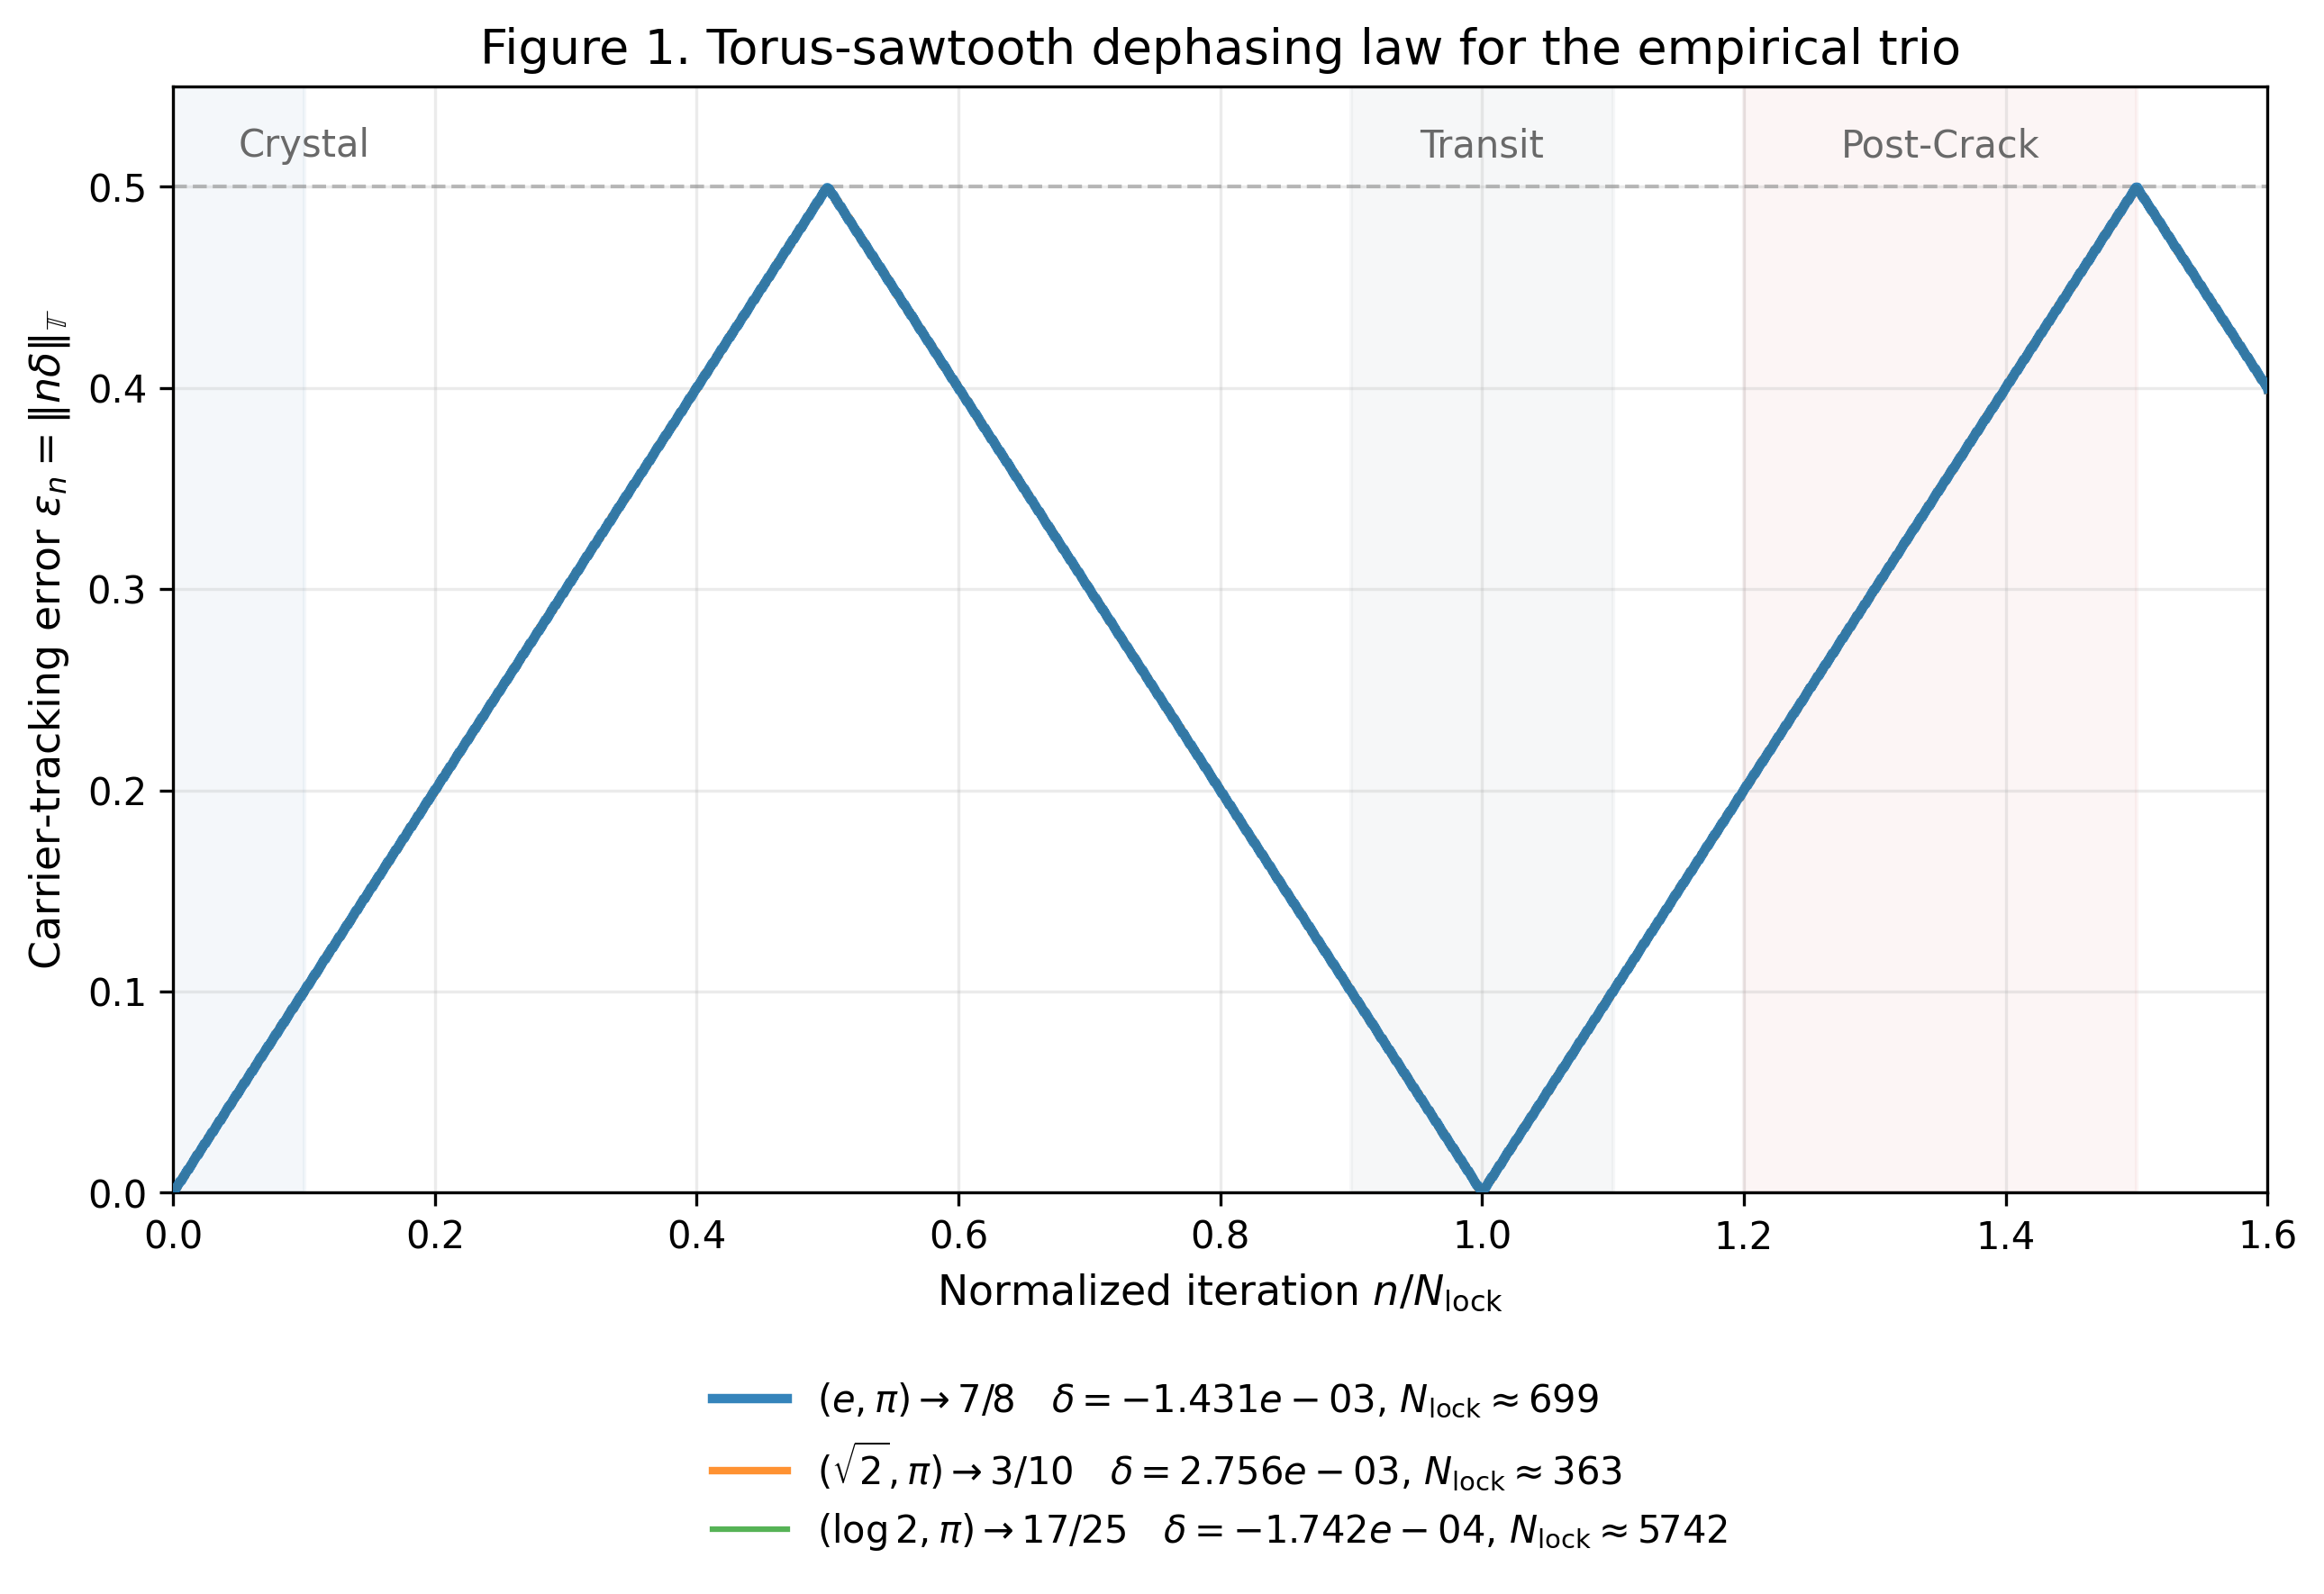
\includegraphics[width=\textwidth]{figure1_sawtooth.png}
    \caption{The torus-sawtooth dephasing law. Carrier-tracking errors $\epsilon_n$ for the empirical trio are plotted against normalized time $n/N_{\mathrm{lock}}$. The shared phase-cycle mechanism of alignment, shear, and wraparound is visually identical across all three scales.}
    \label{fig:sawtooth}
\end{figure}

\begin{figure}[p]
    \centering
    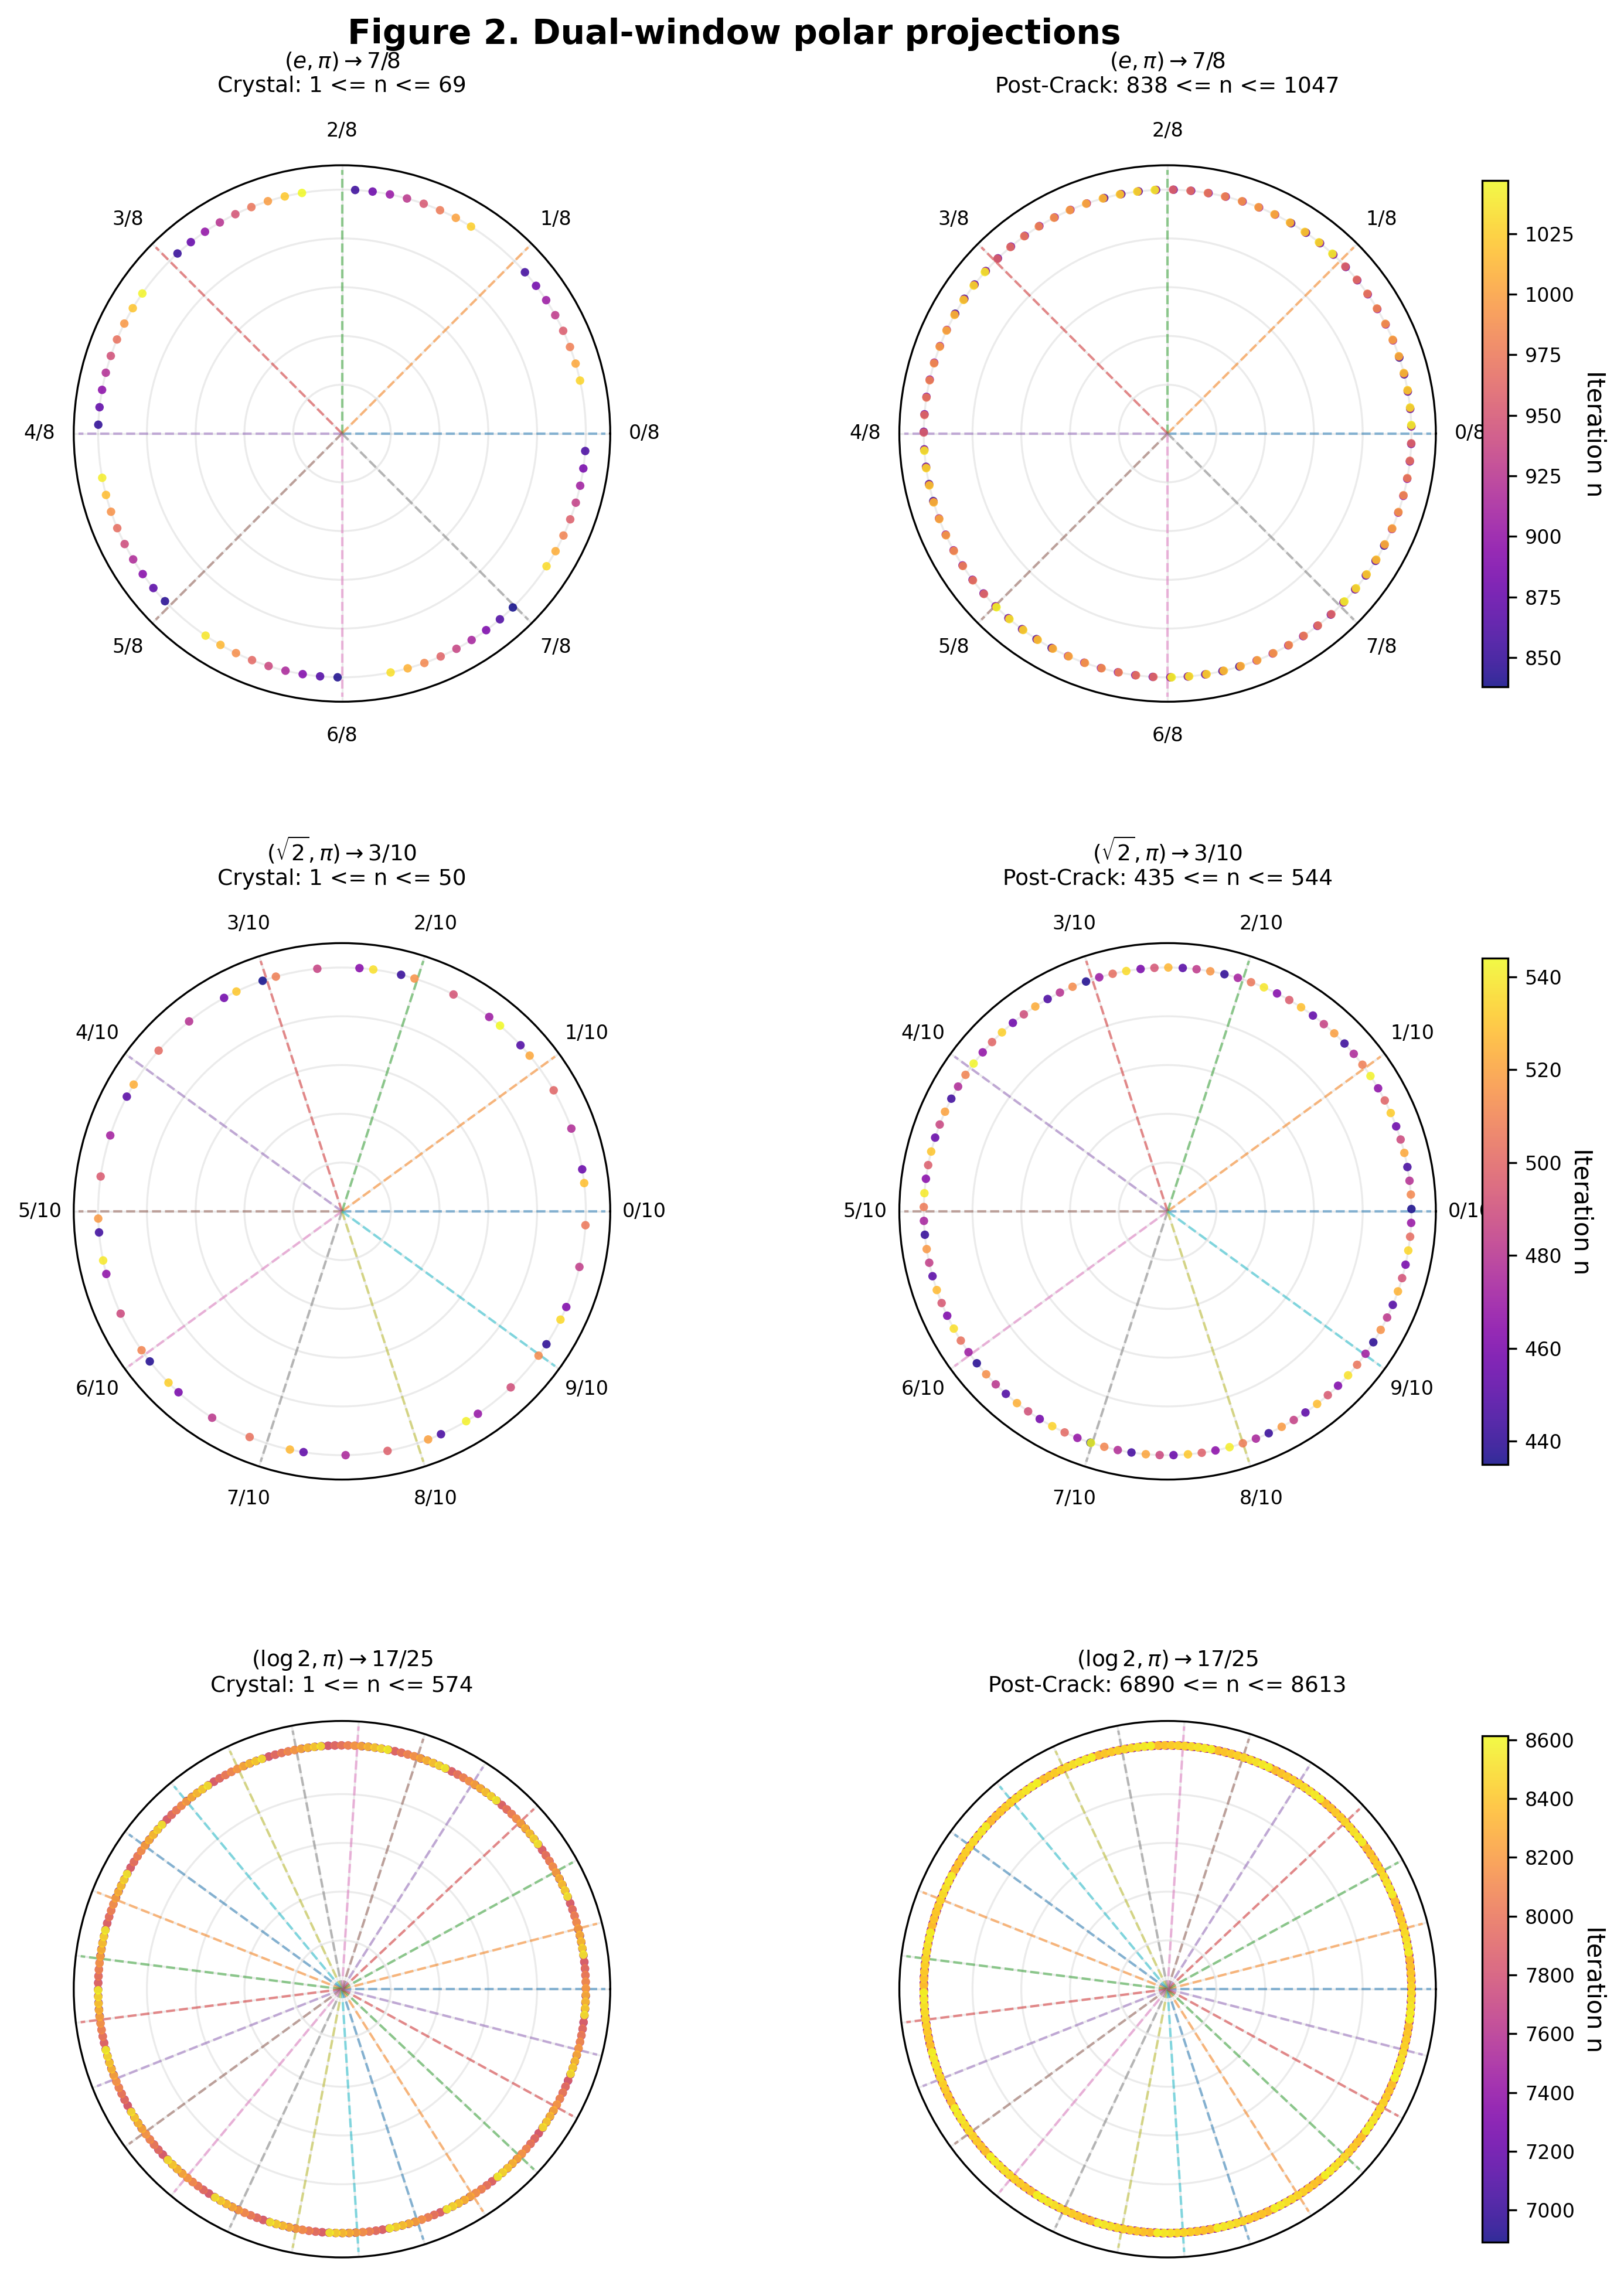
\includegraphics[width=0.95\textwidth]{figure2_polar_trio.png}
    \caption{Dual-window polar projections comparing the initial crystal alignment to the post-crack shear regime. The visible degradation of symmetry in each case is the direct geometric consequence of the dephasing term $\delta$.}
    \label{fig:polar}
\end{figure}

\section{Conclusion}

This paper has reformulated apparent modular geometric structure as a problem in arithmetic dynamics. For a pair of positive constants $(\alpha,\beta)$, the modular logarithmic orbit
\[
x_n=\{n\rho(\alpha;\beta)\},
\qquad
\rho(\alpha;\beta)=\left\{\frac{\log \alpha}{\log \beta}\right\},
\]
exhibits transient $q$-sector geometries whenever the rotation number $\rho$ is well approximated by a rational carrier $p/q$. The governing law is exact:
\[
\epsilon_n^{(p/q)}
=
d_{\T}\!\left(x_n,\left\{\frac{np}{q}\right\}\right)
=
\lVert n(\rho-p/q)\rVert_{\T}.
\]
Thus the observed geometry is not an independent structural object. It is the visible trace of rational shadowing under a toral phase-drift law.

The principal conceptual shift of the framework is therefore a shift from symbolic interpretation to measurable mechanism. Apparent octagons, decagons, and higher-order sector patterns are not treated here as evidence of hidden physical ontology or privileged numerical design. They are transient manifestations of exact rational carriers modulated by a dephasing error $\delta=\rho-p/q$. The characteristic scale $N_{\mathrm{lock}}=1/|\delta|$ is accordingly not a terminal breakdown point, but the natural period of a torus-sawtooth dephasing cycle.

A second conclusion concerns the role of discrete modulus. The modulus $M$ does not compose the geometry. It discretizes it. Proposition~3.1 shows that the normalized lane error differs from the intrinsic torus error by at most a mesh term of order $1/M$. Consequently, highly composite moduli may sharpen or blur the visual rendering of a transient symmetry, but they do not generate that symmetry. In particular, the historical prominence of specific moduli should be interpreted as a property of display quality and arithmetic commensurability, not as evidence of a special dynamical source.

The empirical trio $(e,\pi)\to 7/8$, $(\sqrt{2},\pi)\to 3/10$, and $(\log 2,\pi)\to 17/25$ illustrates three aspects of the same law: a visually legible low-denominator transient, a mid-denominator bridge case reaching the shear-dominated regime on a substantially shorter timescale, and a high-denominator case whose arithmetic coherence outstrips unaided visual recognition. In each case, the observed transient symmetry is predicted in advance by a strong rational approximant to the rotation number, rather than inferred retrospectively from the projection. Taken together, these examples support a general program in which constants are characterized by spectral fingerprints: continued-fraction structure, dominant rational carriers, dephasing scales, and modulus-robust shadowing profiles.

Several natural directions remain. One is the systematic classification of transient geometries by continued-fraction convergents and semiconvergents of $\rho$. Another is the study of coherence statistics and break criteria adapted to denominator scale. A third is the extension of the present framework from selected examples to large atlases of constants and bases. In each case, the emphasis should remain on prediction from Diophantine structure rather than retrospective pattern recognition.

The central message is therefore modest but precise: modular logarithmic geometry is real, but it is descriptive rather than ontological. Its patterns are the transient shadows cast by rational approximation on irrational rotation. The fog resolves not into metaphysics, but into mechanics.

\end{document}
